In order to test the final system against the requirements set out in
section \ref{design:reqs}, the team decided to produce a
questionnaire which would be given to students using the application
for them to give us feedback.
The raw data for this feedback is shown in appendix
\ref{app:questionnaireResponses}.

While other methods of testing exist (e.g. experimental) it was felt
that with the time constraints in place we would not be able to run a
test requiring our direct involvement and that we would receive more
data from a questionnaire.

%---------------------------------------------------------------------
\subsection{Questionnaire System}

Many questionnaire services exist on the internet, such as
SurveyMonkey \cite{surveyMonkey}, FreeOnlineSurveys
\cite{freeOnlineSurveys}, and Google Docs Forms
\cite{googleDocsForms}.

The team decided to use the Google Form, simply because most members
of the team have a Google account, and because it was free.

On closer inspection it could also export its responses to a Google
Docs Spreadsheet which itself could be exported to a variety of
formats.

%---------------------------------------------------------------------
\subsection{Questions}

Generally, the questionnaire needed to be as concise as possible to
avoid any data being corrupted by frustration at the questionnaire.
To this end we kept the number of questions in general to a minimum
and only asked for a description if it was necessary.

\subsubsection{Skill Level}
At the demonstration, the team realised that not every user will be in
the expected age bracket of 18 to 20-years-old who have used computers
their entire lives.
This led to the decision that the feedback should take the user's age
into account, to ensure that there are no patterns in the data
suggesting a particular age group struggles with the application.

In addition, we ask the user for their ``Confidence'' with computers
in general, on a scale from 0 to 5 ie no middle option so there has
to be a bias to confident or not confident.
This completely subjective question should allow us to see if people
who perhaps do not use computers on a daily basis handle the
application, since we believe we made the application (and
accompanying user guide in appendix \ref{app:userGuideCurrent}) as
user-friendly as possible.

We are also aware of some colour-use in the program that could be
problamatic for colour-blind people so we ask the user if they are or
not.

To get an idea of the user's knowledge of primer design, we ask the
user for their self-assessed understanding before using the system, on
a 0 to 5 scale.

All of this data provides us with the baseline skill level with
computers and with primer design of the user, before they use the
system.

\subsubsection{User's Experience with the System}
The following questions were designed to provide us with feedback on
the user's experience with the system.

The first of these follows the self-assessed understanding of primer
design before using the system, with a self-assessed understanding
after using the system, on the same scale.
This will provide us with test data towards the requirement to teach
students about primer design and PCR.

Ideally, as discussed in section \ref{design:reqs}, the system would
be used as a revision tool in students' own time and/or in a
laboratory setting with tutors on hand to help the student with any
problems.
To see if we met this requirement, we asked the user if they would use
the system to study one of the following options:
\begin{itemize}
\item Both Primer Design and PCR
\item Just Primer Design
\item Just PCR
\item Neither
\end{itemize}
Which provides the user, and the team, with every possible answer to
the question, in the most concise way possible.

Following this, we decided to ask the user if they felt they were
given enough information from the application.
In retrospect, this question should have been clearer in that it
should have specified to disregard the user guide.
We wanted to ask this to assess how easily people would be able to use
the application without the user guide.

Technical difficulties were fairly common in the demo build (section
\ref{eval:demo}) but since members of the team were present, we could
instantly know about them.
However since the system was now being used from where the user
happened to be, we had no direct way to be told of any technical
issues or bugs.
To this end, we asked the user for any technical issues they found
while using the application.

Lastly, we ask for any further comments, in case the user wanted to
tell us something we had not asked before this point in the
questionnaire.
To keep it light-hearted, we recommended telling us a joke in the
description of the question, needless to say we had some interesting
feedback for this particular question.

%---------------------------------------------------------------------
\subsection{Feedback Analysis}

In total we received 15 responses, see appendix
\ref{app:questionnaireResponses} for the raw data.
These responses have yielded some interesting results with a few
anomalies.

\subsubsection{Learning}

Of course, the main objective of the system is to help users revise or
solidify the idea of primer design within PCR, if we have not managed
this, we have failed our users.

\begin{figure}[h]
  \begin{center}
    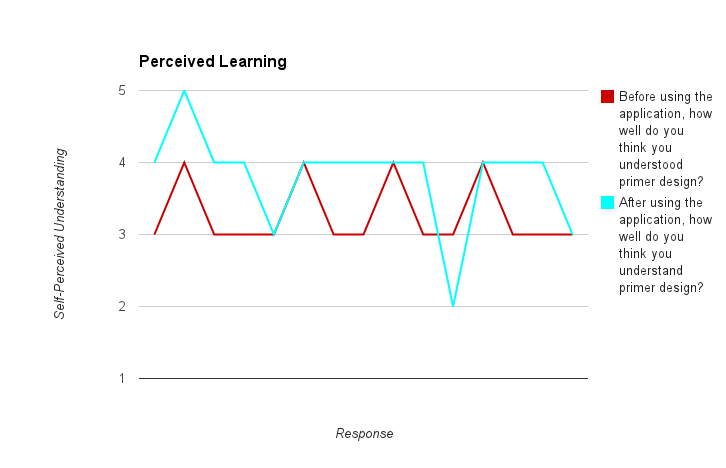
\includegraphics[width=\textwidth]{./images/perceivedLearning.png}
    \caption{Perceived Learning Chart}
    \label{fig:feedbackAnalysis:perceivedLearning}
  \end{center}
\end{figure}

If the application was perfect in this regard and a graph was plotted
for response against score given to the ``Before'' and ``After''
understanding questions, the graph would show that the ``After''
responses line was consistently above the ``Before'' line, implying
that users always see an improvement in understanding.
Unfortunately, as can be seen in figure
\ref{fig:feedbackAnalysis:perceivedLearning} which used the data in
appendix \ref{app:questionnaireResponses}, this is currently not the
case.

One third of responses stated that their understanding of primer
design stayed the same before and after using the system and, more
concerningly, one response claimed that using the system reduced their
understanding.
This still means that a majority of users, 60\% of users who responded
to the questionnaire, found using the system increased their
understanding, however this still implies that 40\% of users did not
see an improvement in understanding.

On closer inspection of the users who saw no improvement and stated
that they would not use the system for studying primer design or PCR,
only one gave additional information as to their problem.

This responder stated that they were not confident in how to design
primers and that they expected the system to guide them through the
process.
They go on to say that they had no way of getting additional
information or hints as to how to progress and that there should have
been some way of retrieving this information.
On noting this, the team agreed that, while the ``Primer Design
Rules'' and ``Primer Feedback'' functions of the system were useful to
someone who had a basic understanding of primers, newer users would
struggle since the rules and feedback themselves are not explicit
in telling the user how they can improve their primers, though it is
very heavily implied.
The team agreed that while this was an isolated case, it may have been
the reason for the other responses which stated no improvement in
understanding, and has been added to future work (see chapter
\ref{future}).

\subsubsection{Information From Application}
Most of the responses we received to this question do not directly
answer the question, since we asked for information \textbf{from the
  application} and most responses referred to the user guide.
However, because so many (a third of respondents) state that the user
guide was helpful (see appendix \ref{app:questionnaireResponses}), we
can assume that not enough information was given by the application
itself for a user to comfortably use the system without it (at least
for the first time using it).

The user guide was created on the premise that the application had to
familiarise people with the NCBI website and we could not do this
purely within the application so the user guide would provide this
requirement.
We were also working under the assumption that the student had never
used the NCBI website before.
However, the team wanted to know if people found the information on the
application helpful or whether the user guide could be the sole source
of instruction.

In retrospect this was a null point and due to the wording of the
question we have little data to support the idea of the user being unable
to use the application.
However, one respondent did note that they tried to use the system
without the user guide and did not know how to use the NCBI website
\cite{ncbi} to retrieve a DNA sequence, then read the user guide and
found it very helpful. 

\subsubsection{Technical Difficulties Encountered}

Of the 15 respondents, three mentioned something for the technical
difficulties question.
However, one of these responses was a problem continuing to the next
panel, and does not mention anything suggesting this was a bug and not
simply user error.
Since no other respondent mentioned this, we are considering this as
user error rather than a technical fault.
We therefore have two technical difficulties to consider.

Firstly, one respondent noted that if the user was to enter the
sequence as capital letters instead of lower case, the highlighting
would not appear.
This is a simple problem but one we intend to fix at the earliest
opportunity, as noted in the Future Work chapter (chapter
\ref{future}).
This respondent also comments that the animation does not appear
correctly on their screen and helpfully gives us the resolution of
their screen, namely 1366 x 768 pixels.
Given that the height of the animation was 768, rather than the 600
used by the rest of the system, and that a small number of pixels are
used for most operating systems' equivalent of a taskbar, this is
perfectly understandable and is a known issue.
Unfortunately the animation is hard-coded to be 768 pixels high and
would require a rather large overhaul to fix and is not something we
intend to fix.

Lastly, another respondent stated that the animation ``\ldots did not
run.'' on a University PC.
Unfortunately, with no specification of operating system or other
circumstances this will be difficult to recreate, although the team
intend to investigate this further (as discussed in chapter
\ref{future}).

\subsubsection{Shortfalls of the Questionnaire}
We received no data to insinuate that a particular age group had
problems with the application, with only 3 responders stating that
their age was higher than 20, each with varying base skill level and
responses.
Therefore we do not have enough data to suggest an age-related
correlation.

None of the reponding users stated that they were colour blind, so we
are unable to state that colour blind people would be able to use the
system as easily as those who are not.

The question regarding information from the application was evidently
unclear to the students who frequently responded by talking about the
user guide, rather than the application.
This should have been clarified and perhaps a separate question was
needed for the user guide itself.

